\documentclass[../BachelorAssignment.tex]{subfiles}


\begin{document}
\graphicspath{{\subfix{../Images/}}}

\begin{figure}[H]
    \centering
    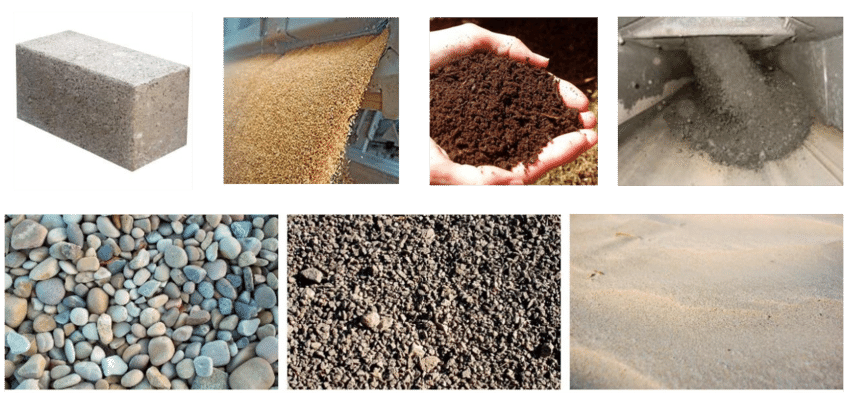
\includegraphics[scale=0.5]{granularExample.png}
    \caption{Examples of Granular Materials.\cite{granularExample}}
    \label{fig:granularExample}
\end{figure}


Granular material is a family of material characterized by its large bulk of densely packed particles, ranging from nanometers to centimeters \cite{introGranular2}, and is able to resist deformation and form heaps, i.e., behave like a solid and withstand strong shear force \cite{introGranular3}. Simple examples of granular materials include sand, gravel, clays, seeds, nuts, and all ranges of powders such as coffee powder, cement powder, which is shown in figure \ref{fig:granularExample}. Furthermore, many processes and equipments in chemical plants use granular materials, such as catalysis, adsorption, and heat exchangers. Granular materials are projected to make about half of the products and three-quarters of the raw materials used in the chemical industry \cite{introGranular}. Thus, understanding how granular materials behave is of great significance. 


Granular material's bulk mechanical behavior is simulated using a Discrete Particle Model (DPM, or Discrete Element Method - DEM), which generates the movement of individual particles to capture the macro-scale behavior. The DPM is a family of numerical methods for computing the motion of a large number of particles \cite{Weng:2015}. Since the properties of granular materials differ wildly, these simulations require an extensive calibration process designed individually for each type of granular material. Some parameters of the granular material model can be measured directly, such as size distribution or density. However, other parameters are effective parameters (i.e., they result from a simplified particle model) and thus cannot be directly measured. These parameters are then calibrated by choosing a few standard calibration setups (rotating drum, heap test, ring shear cell) and simulating these setups in a DPM simulation, and the missing parameters are determined such that the response of the experimental and simulation setups match. This has been done using a Convolutional Neural Network \cite{nn-calibration}, Genetic Algorithm \cite{ga-calibration}, and a recursive Bayesian sequential Monte-Carlo filtering algorithm named GrainLearning \cite{grainLearning}. 

%todo cite more NN paper there? 

% However, these methods are very costly in terms of  time and resources, since it requires a large number of DEM simulations. In this research assignment, another algorithm will be studied: GrainLearning - a Python-based Bayesian calibration tool developed by H.Cheng et al. \cite{grainLearning}. GrainLearning utilizes the recursive Bayesian algorithm to estimate the uncertainty parameters in DPM. As mentioned above, each model requires extensive calibration, and using GrainLearning can make the calibration process more effective by iteratively searching for the optimized parameters, effectively reducing the number of DEM simulations required.

Artificial Neural Network (ANN) is a set of algorithms that seeks to identify correlations in data utilizing a technique that inspired by the way human brain operates - mimicking how each neurons in the brain signaling each other. The most basic ANN models is the Feedforward Multilayer Perceptron Neural Network (MLPNN), in which the purpose is to define the mapping between the input and output \(y = f(x;\theta)\), and approximate the parameter \(\theta\) which results in the best possible function. In MLPNN, the data will flows in one direction from the input to output, hence the name feedforward. Like other supervised learning algorithms, a MLPNN need to be trained before it can accurately describe the relations between the input and output. This is typically done by feeding the network with pre-labeled data, compare the model's output with the desired output, and update the weights parameter \(\theta\) - a process called backpropagation. In the context of this Assignment, Neural Network (NN) will be used when refering to Feedforward Multilayer Perceptron Neural Network. 


% GrainLearning has been implemented in MercuryDPM and produces satisfactory results in many cases. However, it is far from clear whether the chosen optimization algorithm is optimal, i.e., whether the calibration results in an optimal parameter set and whether the optimum could be reached faster since currently, a calibration process could run for hours. Therefore, the research question here is that: Is there a more efficient way to calibrate the parameters for DEM simulation using GrainLearning?

\end{document}
